\documentclass[../thesis.tex]{subfiles}

\begin{document}

\chapter{System Architecture}

\section{Introduction}

In the \autoref{sec:layers} and \autoref{sec:responsibilities}, the logical layering and the responsibilities of the components were introduced but how they fit together and work in harmony is still a mystery. In this chapter, I will put the pieces of the puzzle together by discussing of the actual architecture of the system and its behaviours with increasing levels of detail. 


\section{Top-level architecture}

The top-level architecture is a simplified architecture where many low-level components are being grouped together and treated as a singular composite component. It is shown in the figure \ref{fig:toplevel}. The following components in the top-level architecture are composite component:

\begin{itemize}
	\item Remote Sensing (See \autoref{sec:remoteSensing})
	\item Backend (See \autoref{sec:backend})
	\item Frontend (See \autoref{sec:frontend})
	\item Real-time (See \autoref{sec:realtime})
	\item Governor (See \autoref{sec:governor})
\end{itemize}


\begin{figure}[!ht]
	\centering
	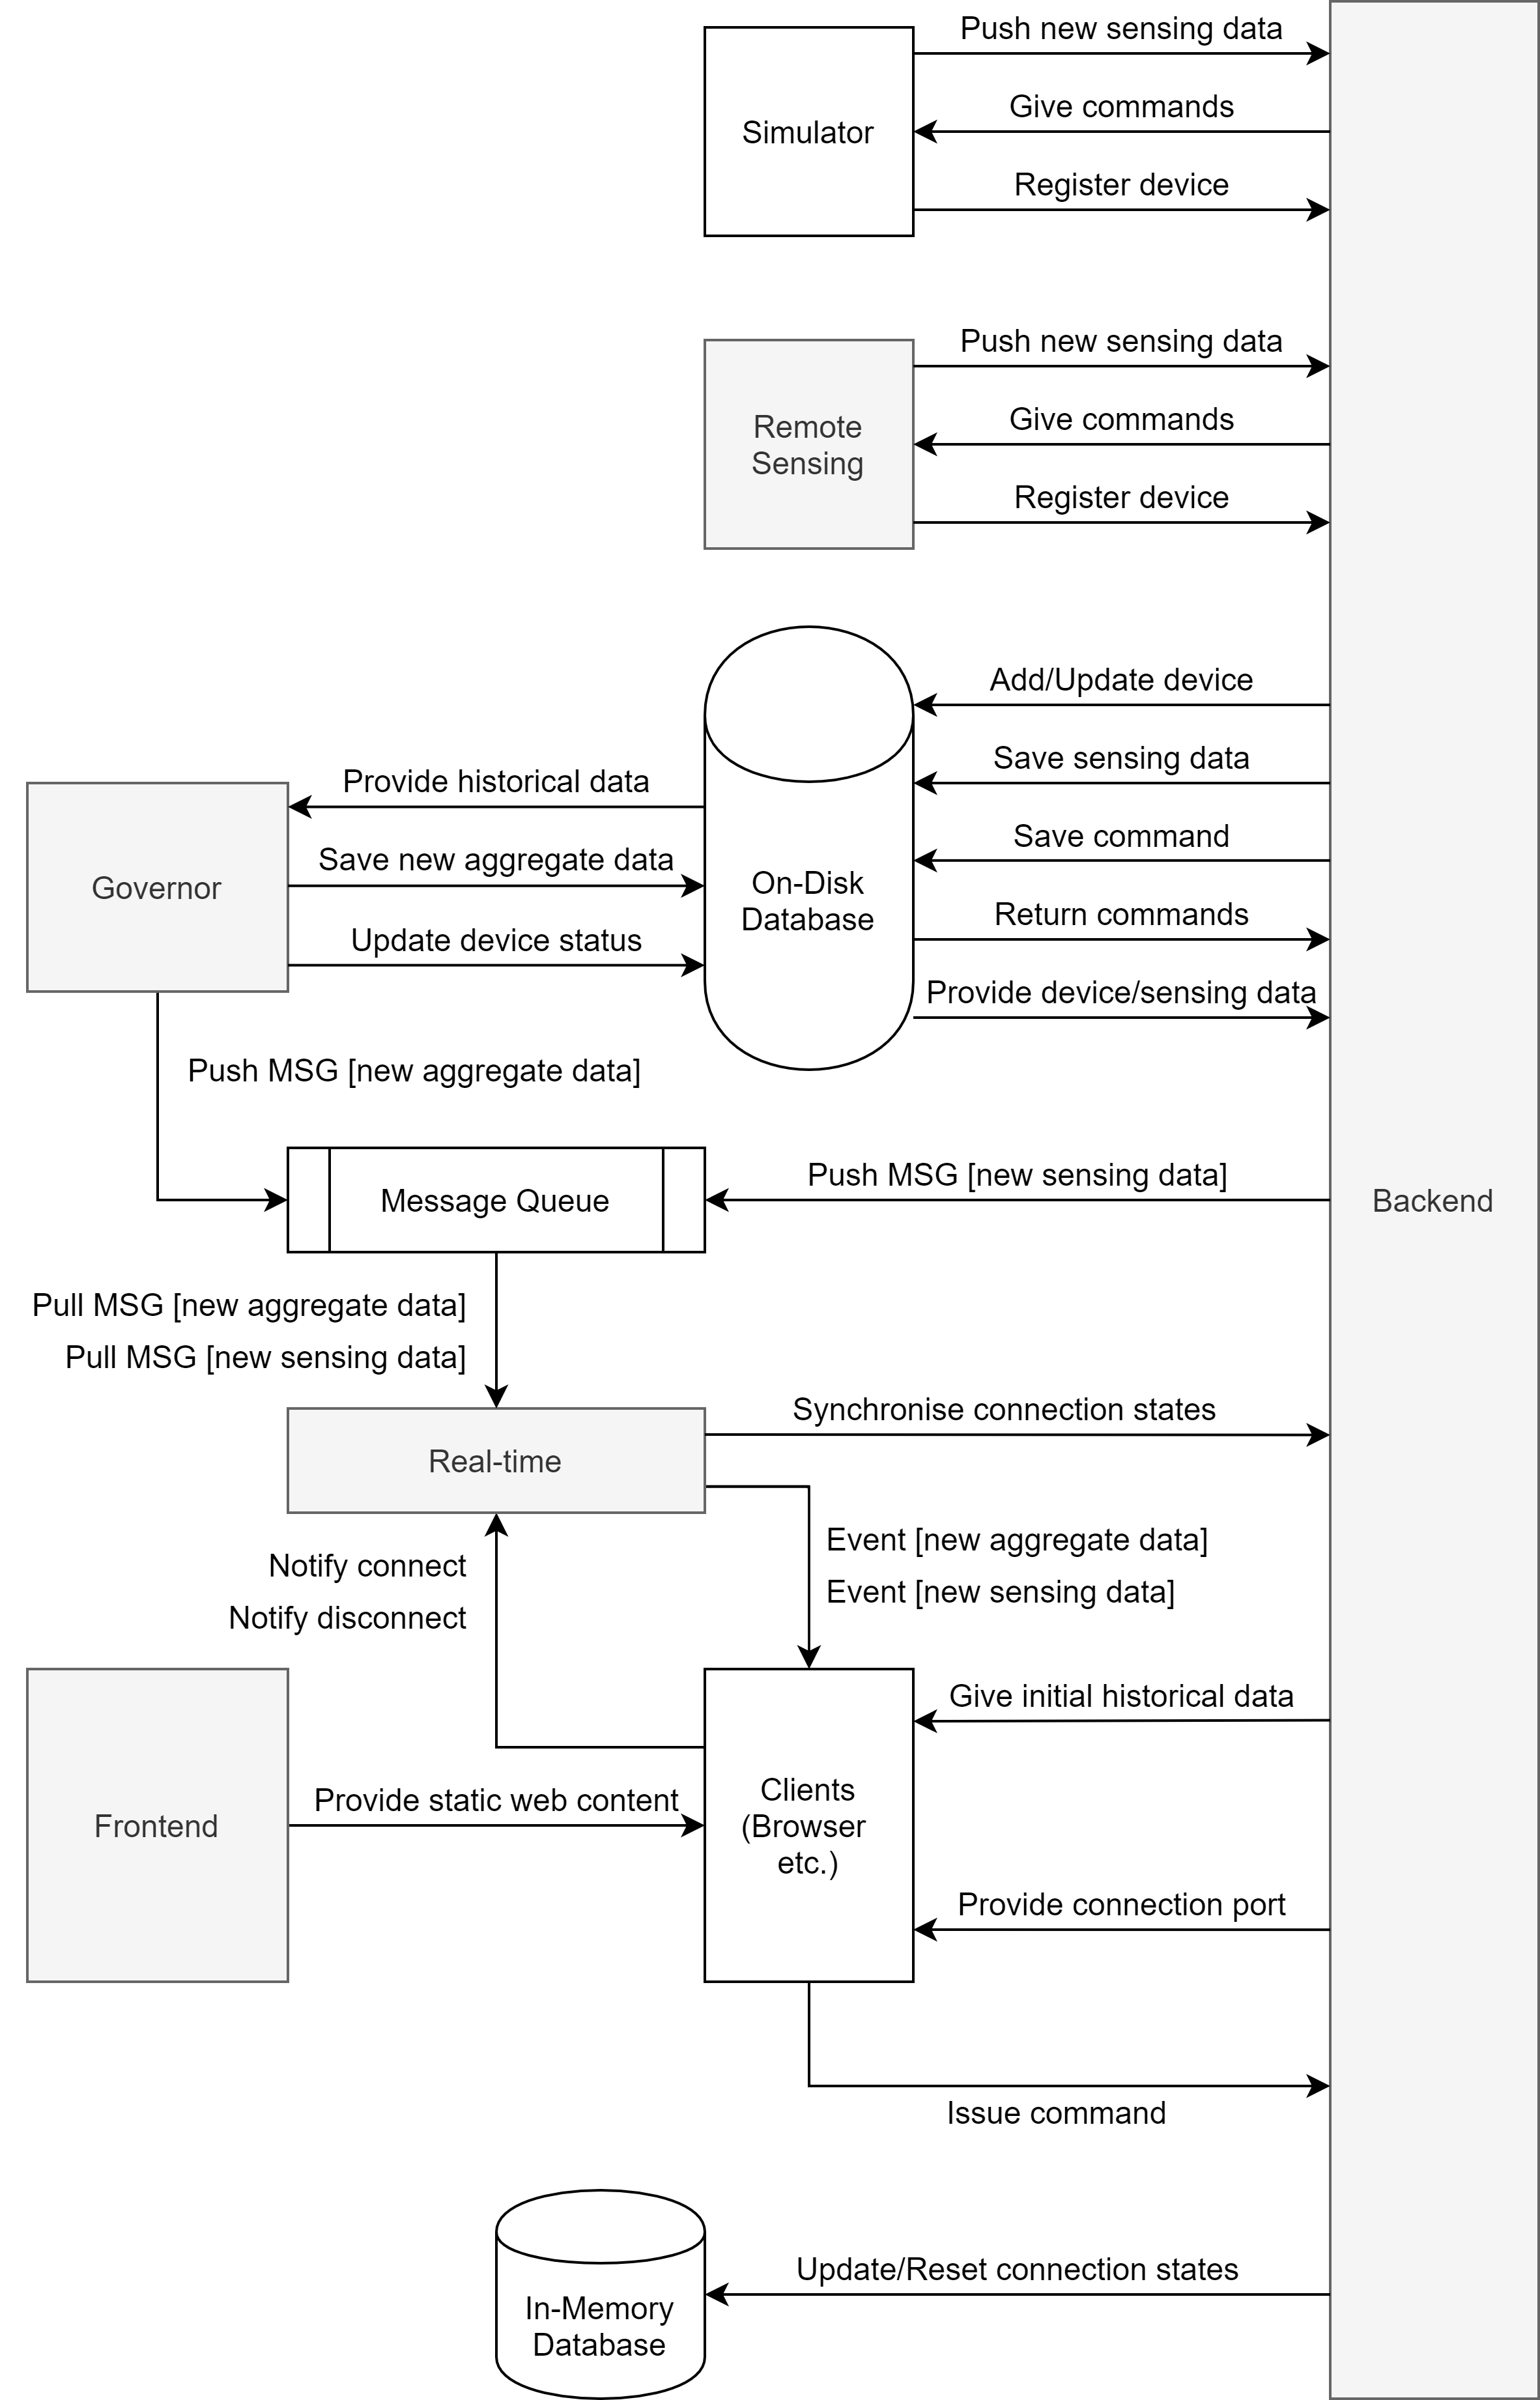
\includegraphics[width=0.84\linewidth]{c4-toplevel.png}
	\caption{Top-level architecture of the proposed system.}
	\label{fig:toplevel}
\end{figure}

\section{Top-level behaviours}

This section provides a general description of how the the proposed system works together with many low-level details abstracted. 

\subsection{Initialisation}

The initialisation process is referring to a device in the remote sensing composite component such as a microcontroller attempting to connect with the server before it can send data and receive commands. When a microcontroller is initialising, it sends a register device request to the backend and then wait for the reply from the backend. Once the request is received by the backend, it tries to find a matching device in the database. If found, then it updates the device status to online. Otherwise, it generates a new device ID, creates a representation of the new device in the database, and set the device status to online. Finally, the backend notifies the microcontroller by returning a response to the initial device registration request, and the intialisation sequence is complete. The figure \ref{fig:init} shows the flow of the initialisation process and the relevant function calls shown in the top-level architecture.

The initialisation process achieves two goals, the first goal is letting the backend knows the device is online and ready to transmit data, and the second goal is getting a unique ID so that it can be identified during the data transmission phase. Once the initialisation process is finished, the microcontroller is ready to transmit data. 

\begin{figure}[!ht]
	\centering
	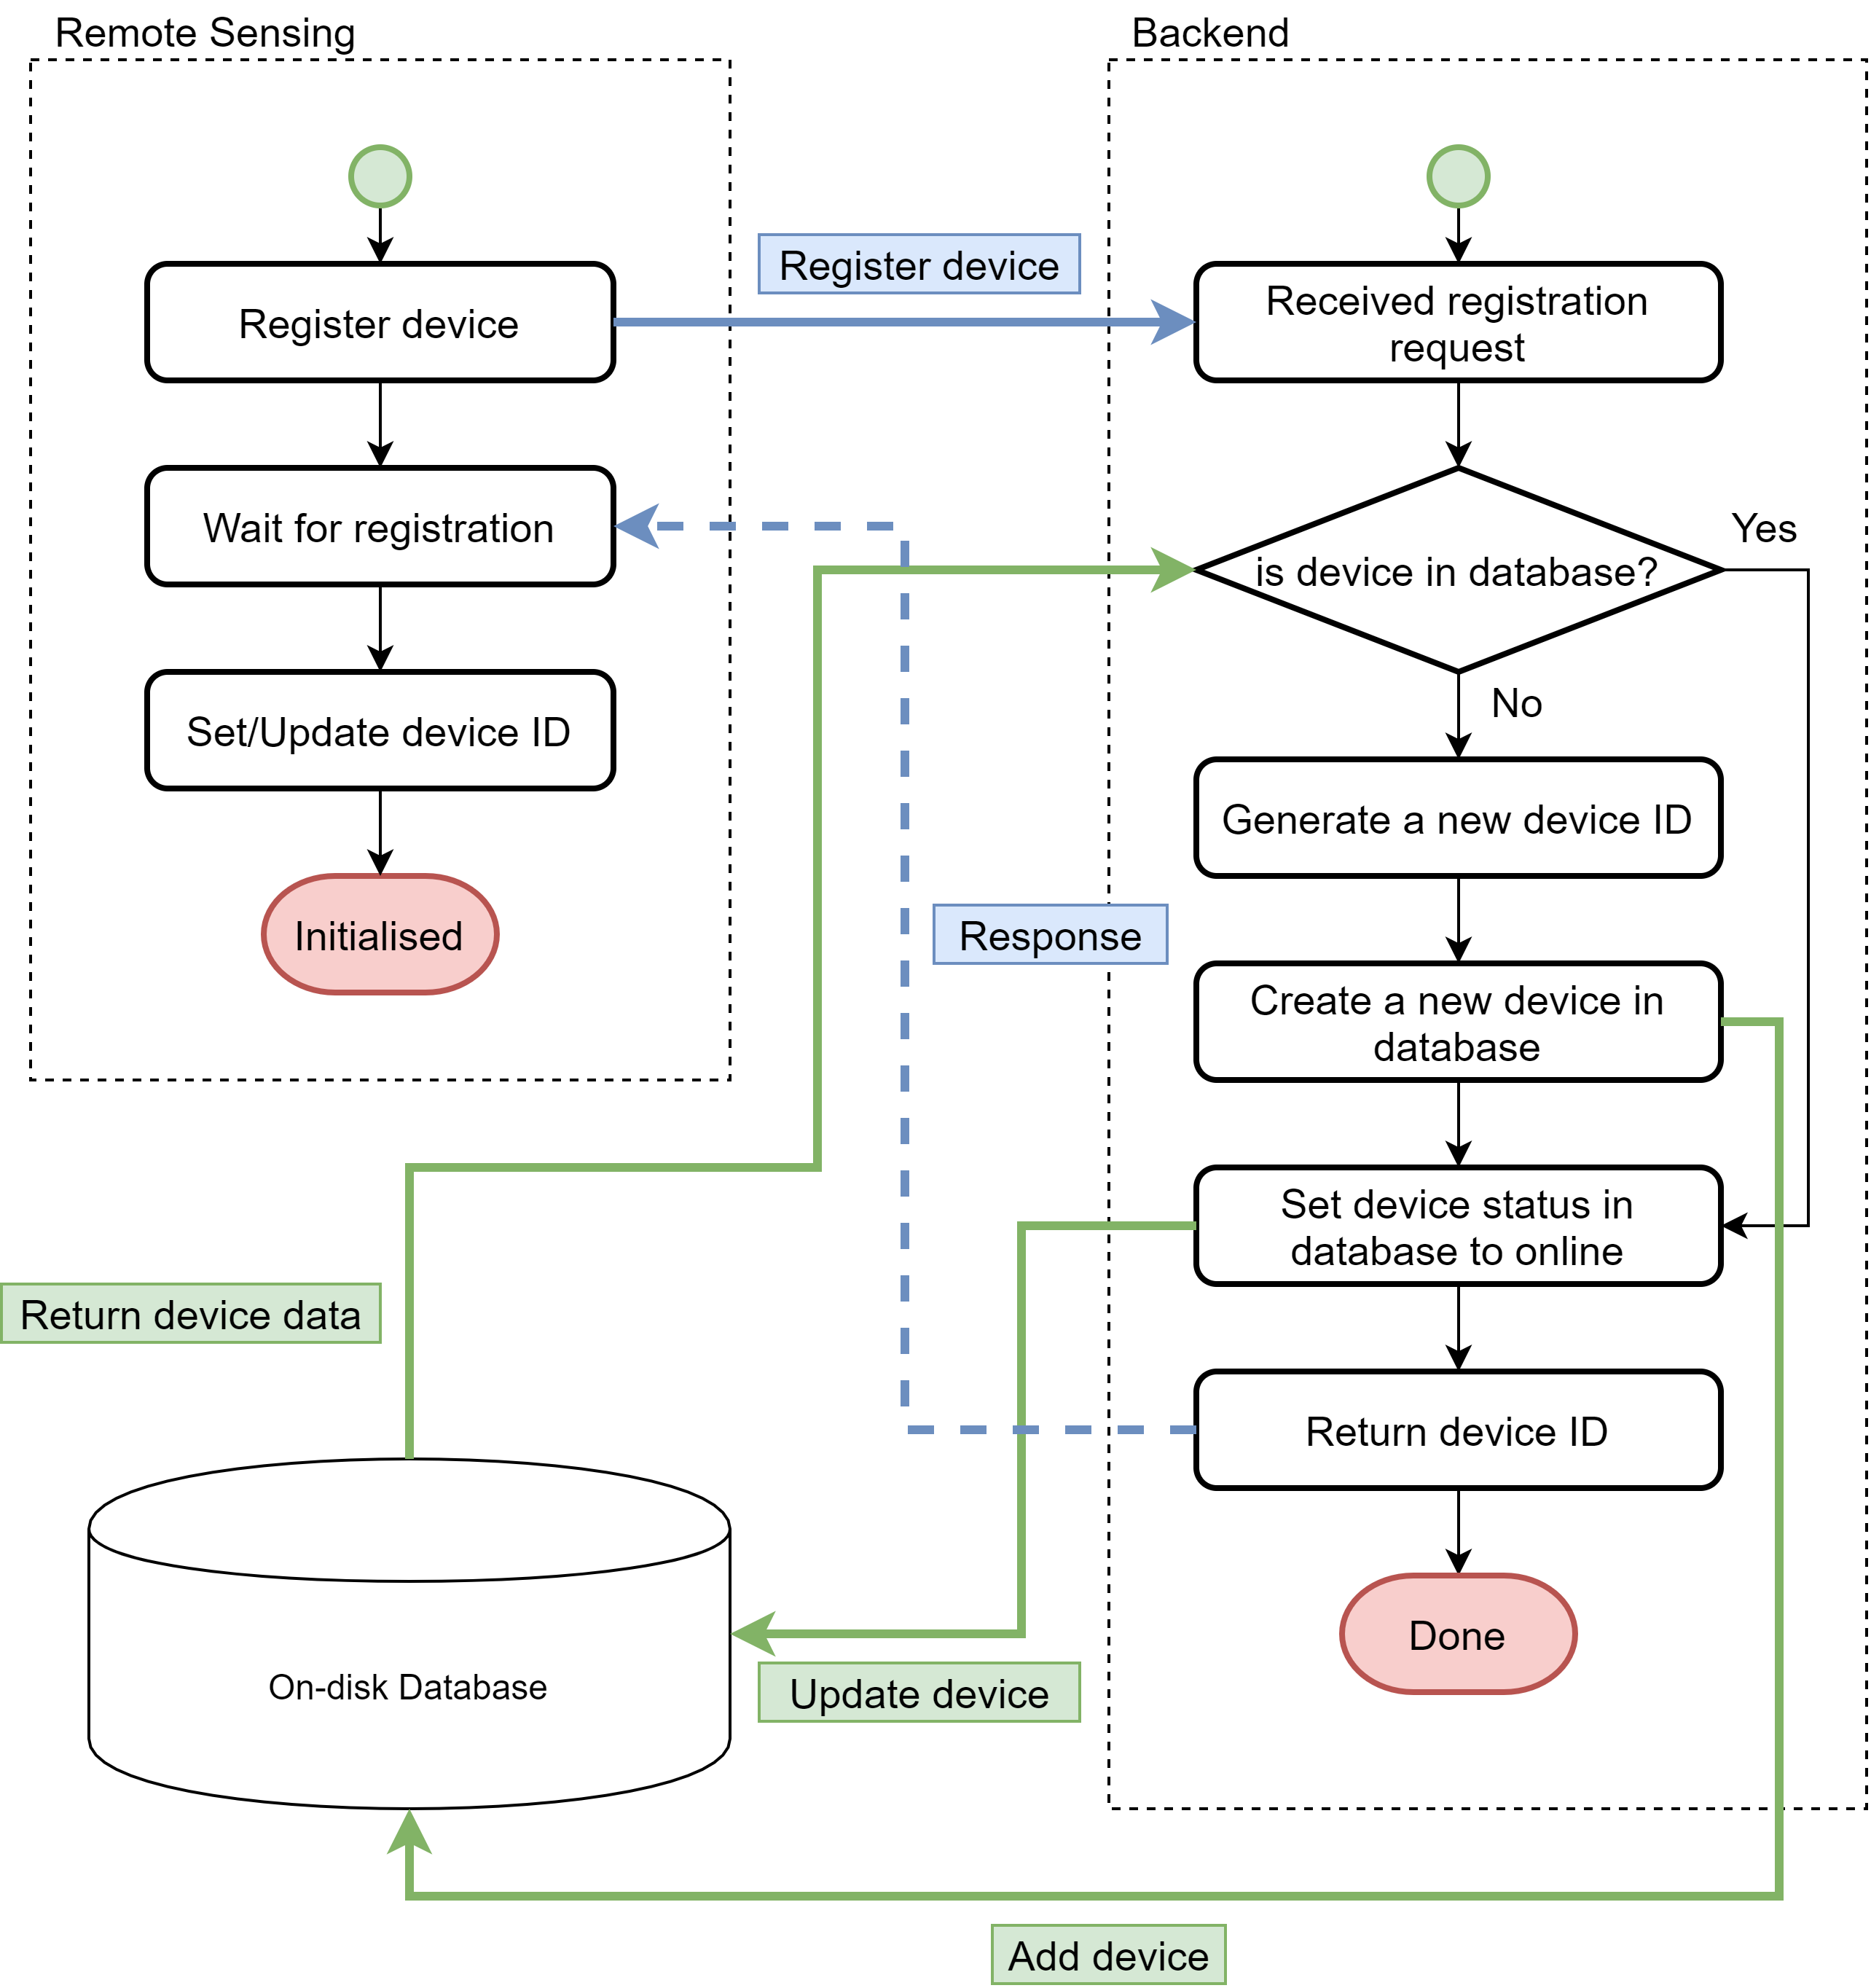
\includegraphics[width=\linewidth]{c4-initialisation.png}
	\caption{The initialisation process.}
	\label{fig:init}
\end{figure}


\subsection{Data recording and device controlling}

The data recording process aims to record data from the sensors and store them into the database. The process begins at the microcontroller where it reads the sensing data from the sensors and then sends it to the backend using the \emph{push new sensing data} request. Once the backend received the sensing data, it begins executing two sequences of instructions simultaneously. The first sequence is used for data recording, where the data is added to the database and then sends a message to clients notifying a new sensing data is available. The second sequence is used for device controlling, where it retrieves a list of commands cumulated in the database, and sends them to the microcontroller through the response to the \emph{push new sensing data} request. As soon as the microcontroller received the commands, it would perform each command in order and wait for 1 second before reading and sending data again. The process is shown in the figure \ref{fig:record}. 

The reason for data recording and device controlling happening at the same time is improving communication efficiency and reducing server load. The microcontroller doesn't need to send two different requests to push data and retrieve commands, which reduces the communication time by half and reduces the number of access to the backend by half. 

Executing two seqeunces of instructions simultaneously has the benefit of reducing the response time of a request. The detailed explanation is provided in \autoref{sec:backend}.

\begin{figure}[!ht]
	\centering
	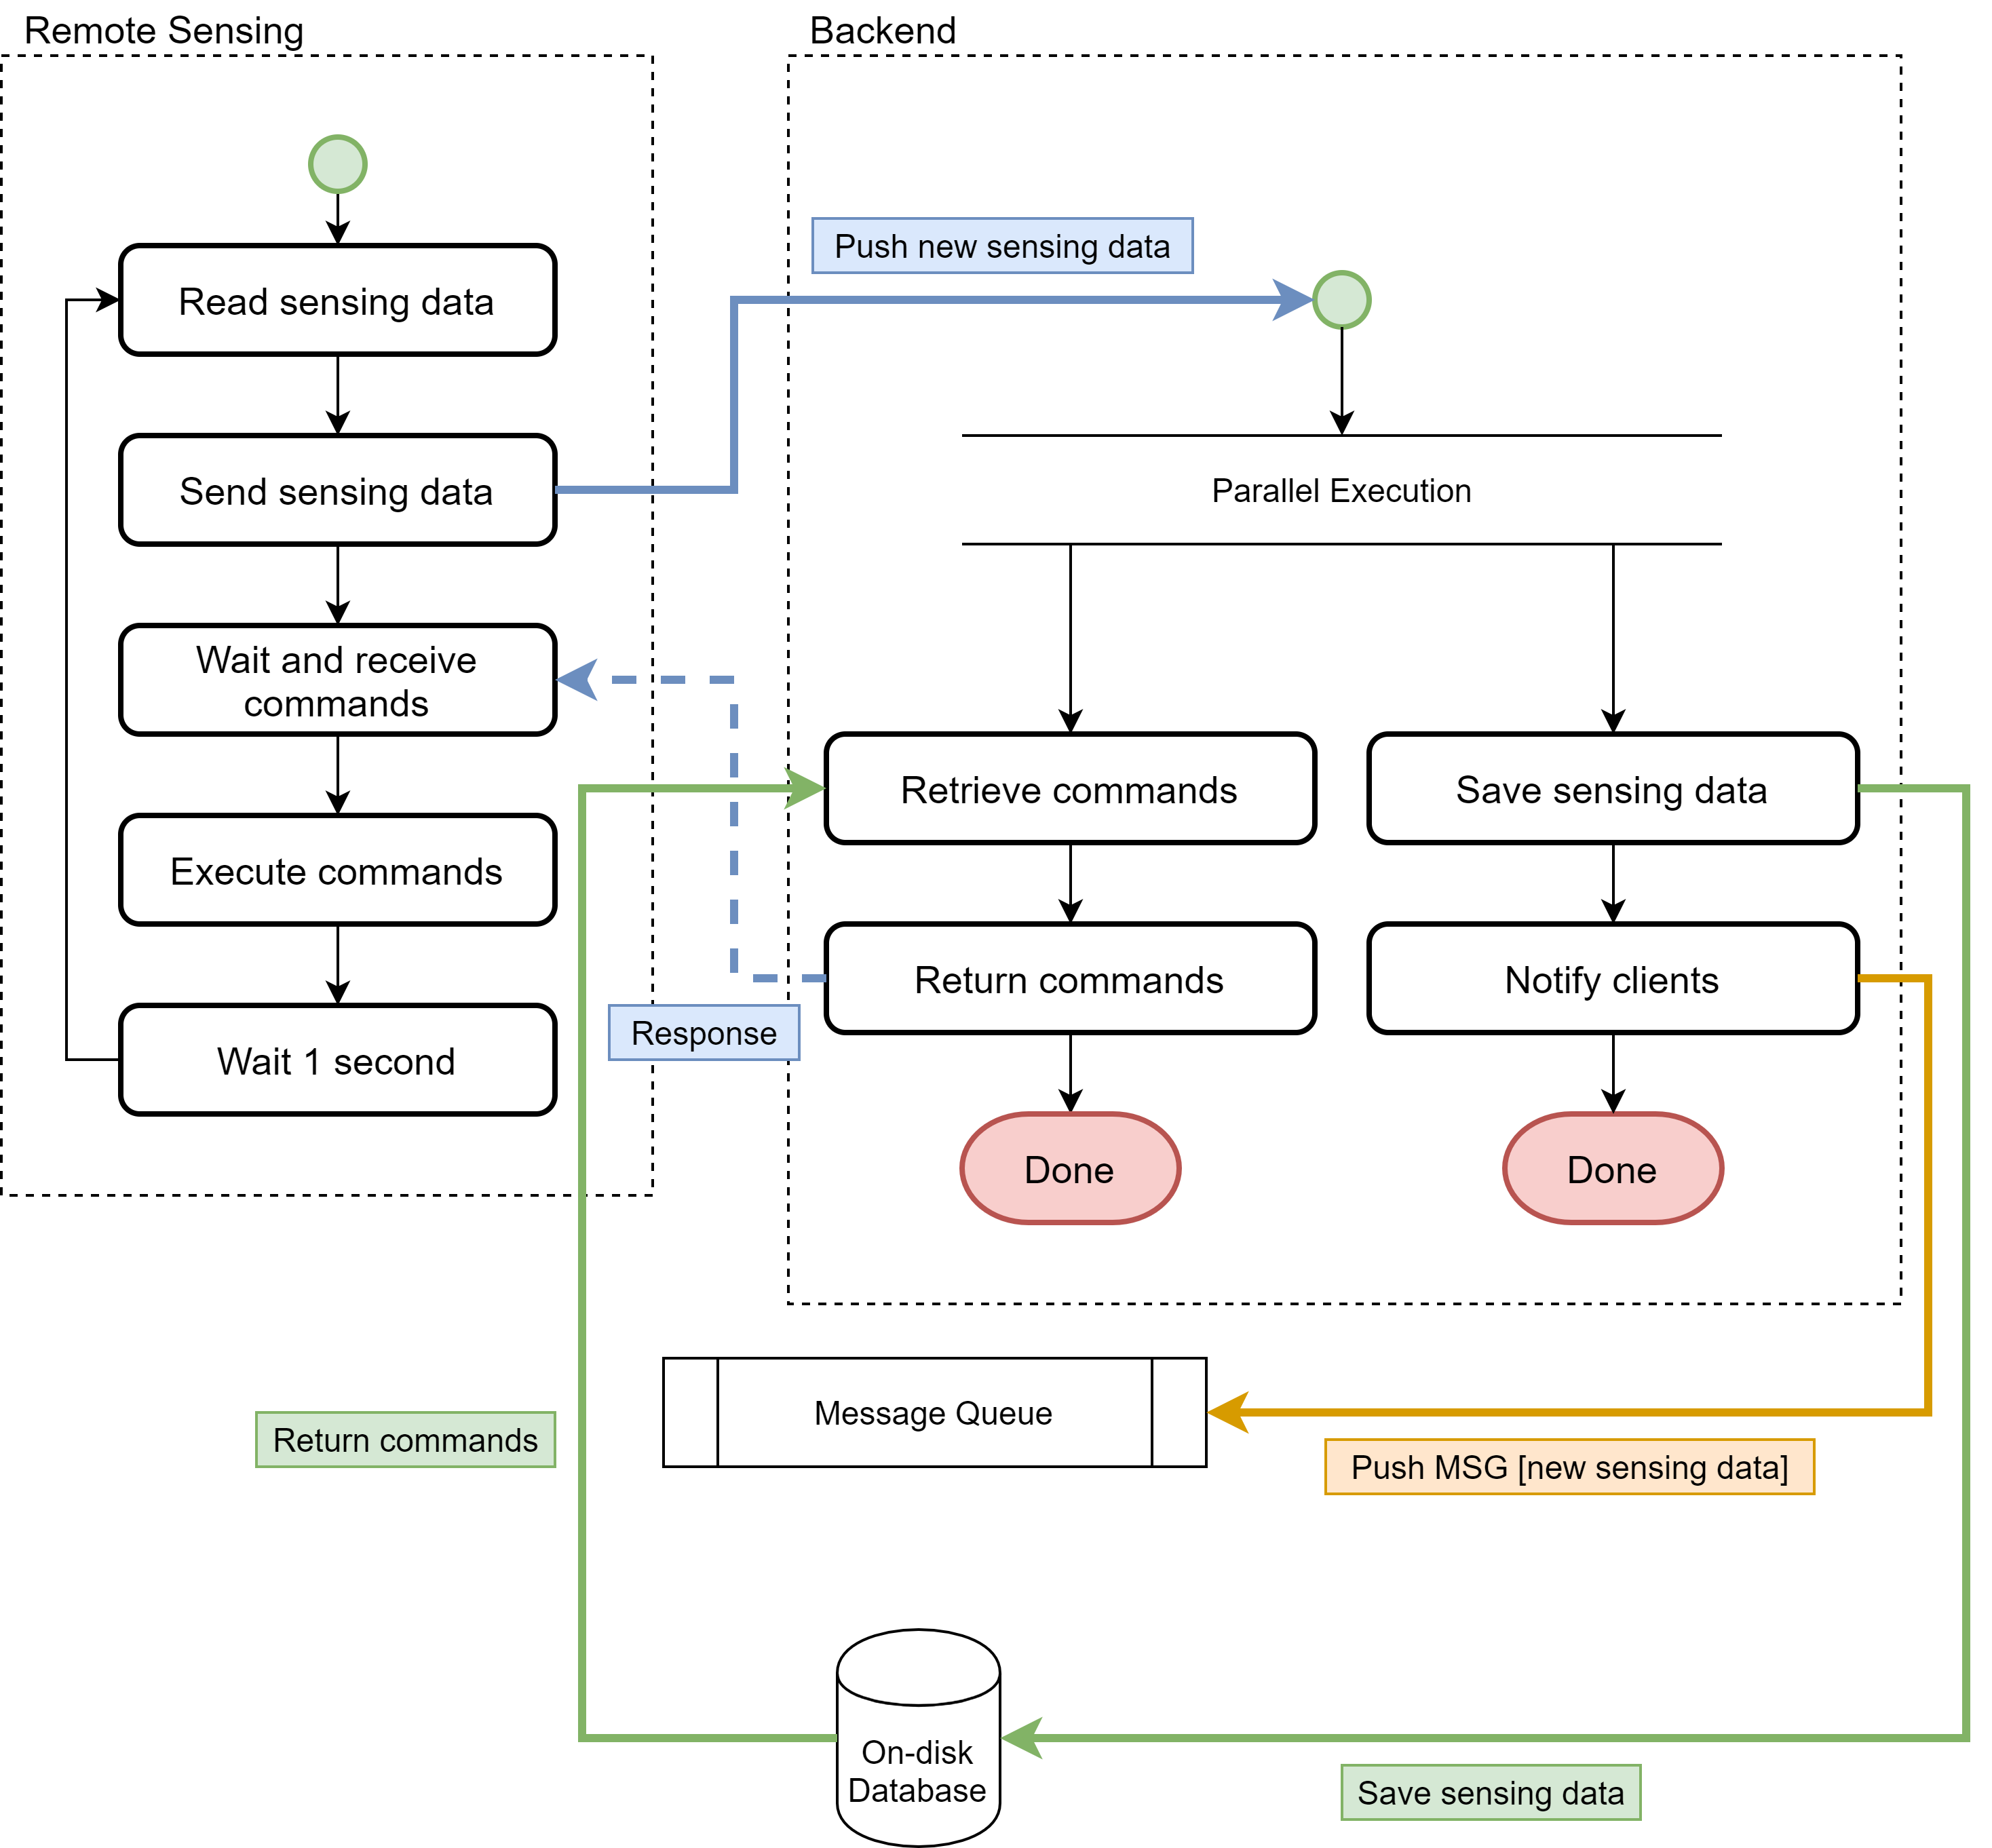
\includegraphics[width=\linewidth]{c4-recording.png}
	\caption{The data recording and device controlling process.}
	\label{fig:record}
\end{figure}

\subsection{Governing}
\label{sec:governor}

Governors are a series of background tasks that are executing periodically and making changes to the system. Currently, there is only one governor in the system, the data aggregation governor.

Every minute, the governor aggregates the sensing data\footnote{The sensing data is also known as the real-time data since it is recorded every second.} for every single device by averaging the sensing data received over the last minute, saving it to the database, and notifying clients about a new aggregate data is available. To prevent the database using too much disk space, it resets the sensing data after aggregation so the number of samples in the sensing data is kept below 60 samples. The governing process is shown in the figure \ref{fig:governing}.

\begin{figure}[!ht]
	\centering
	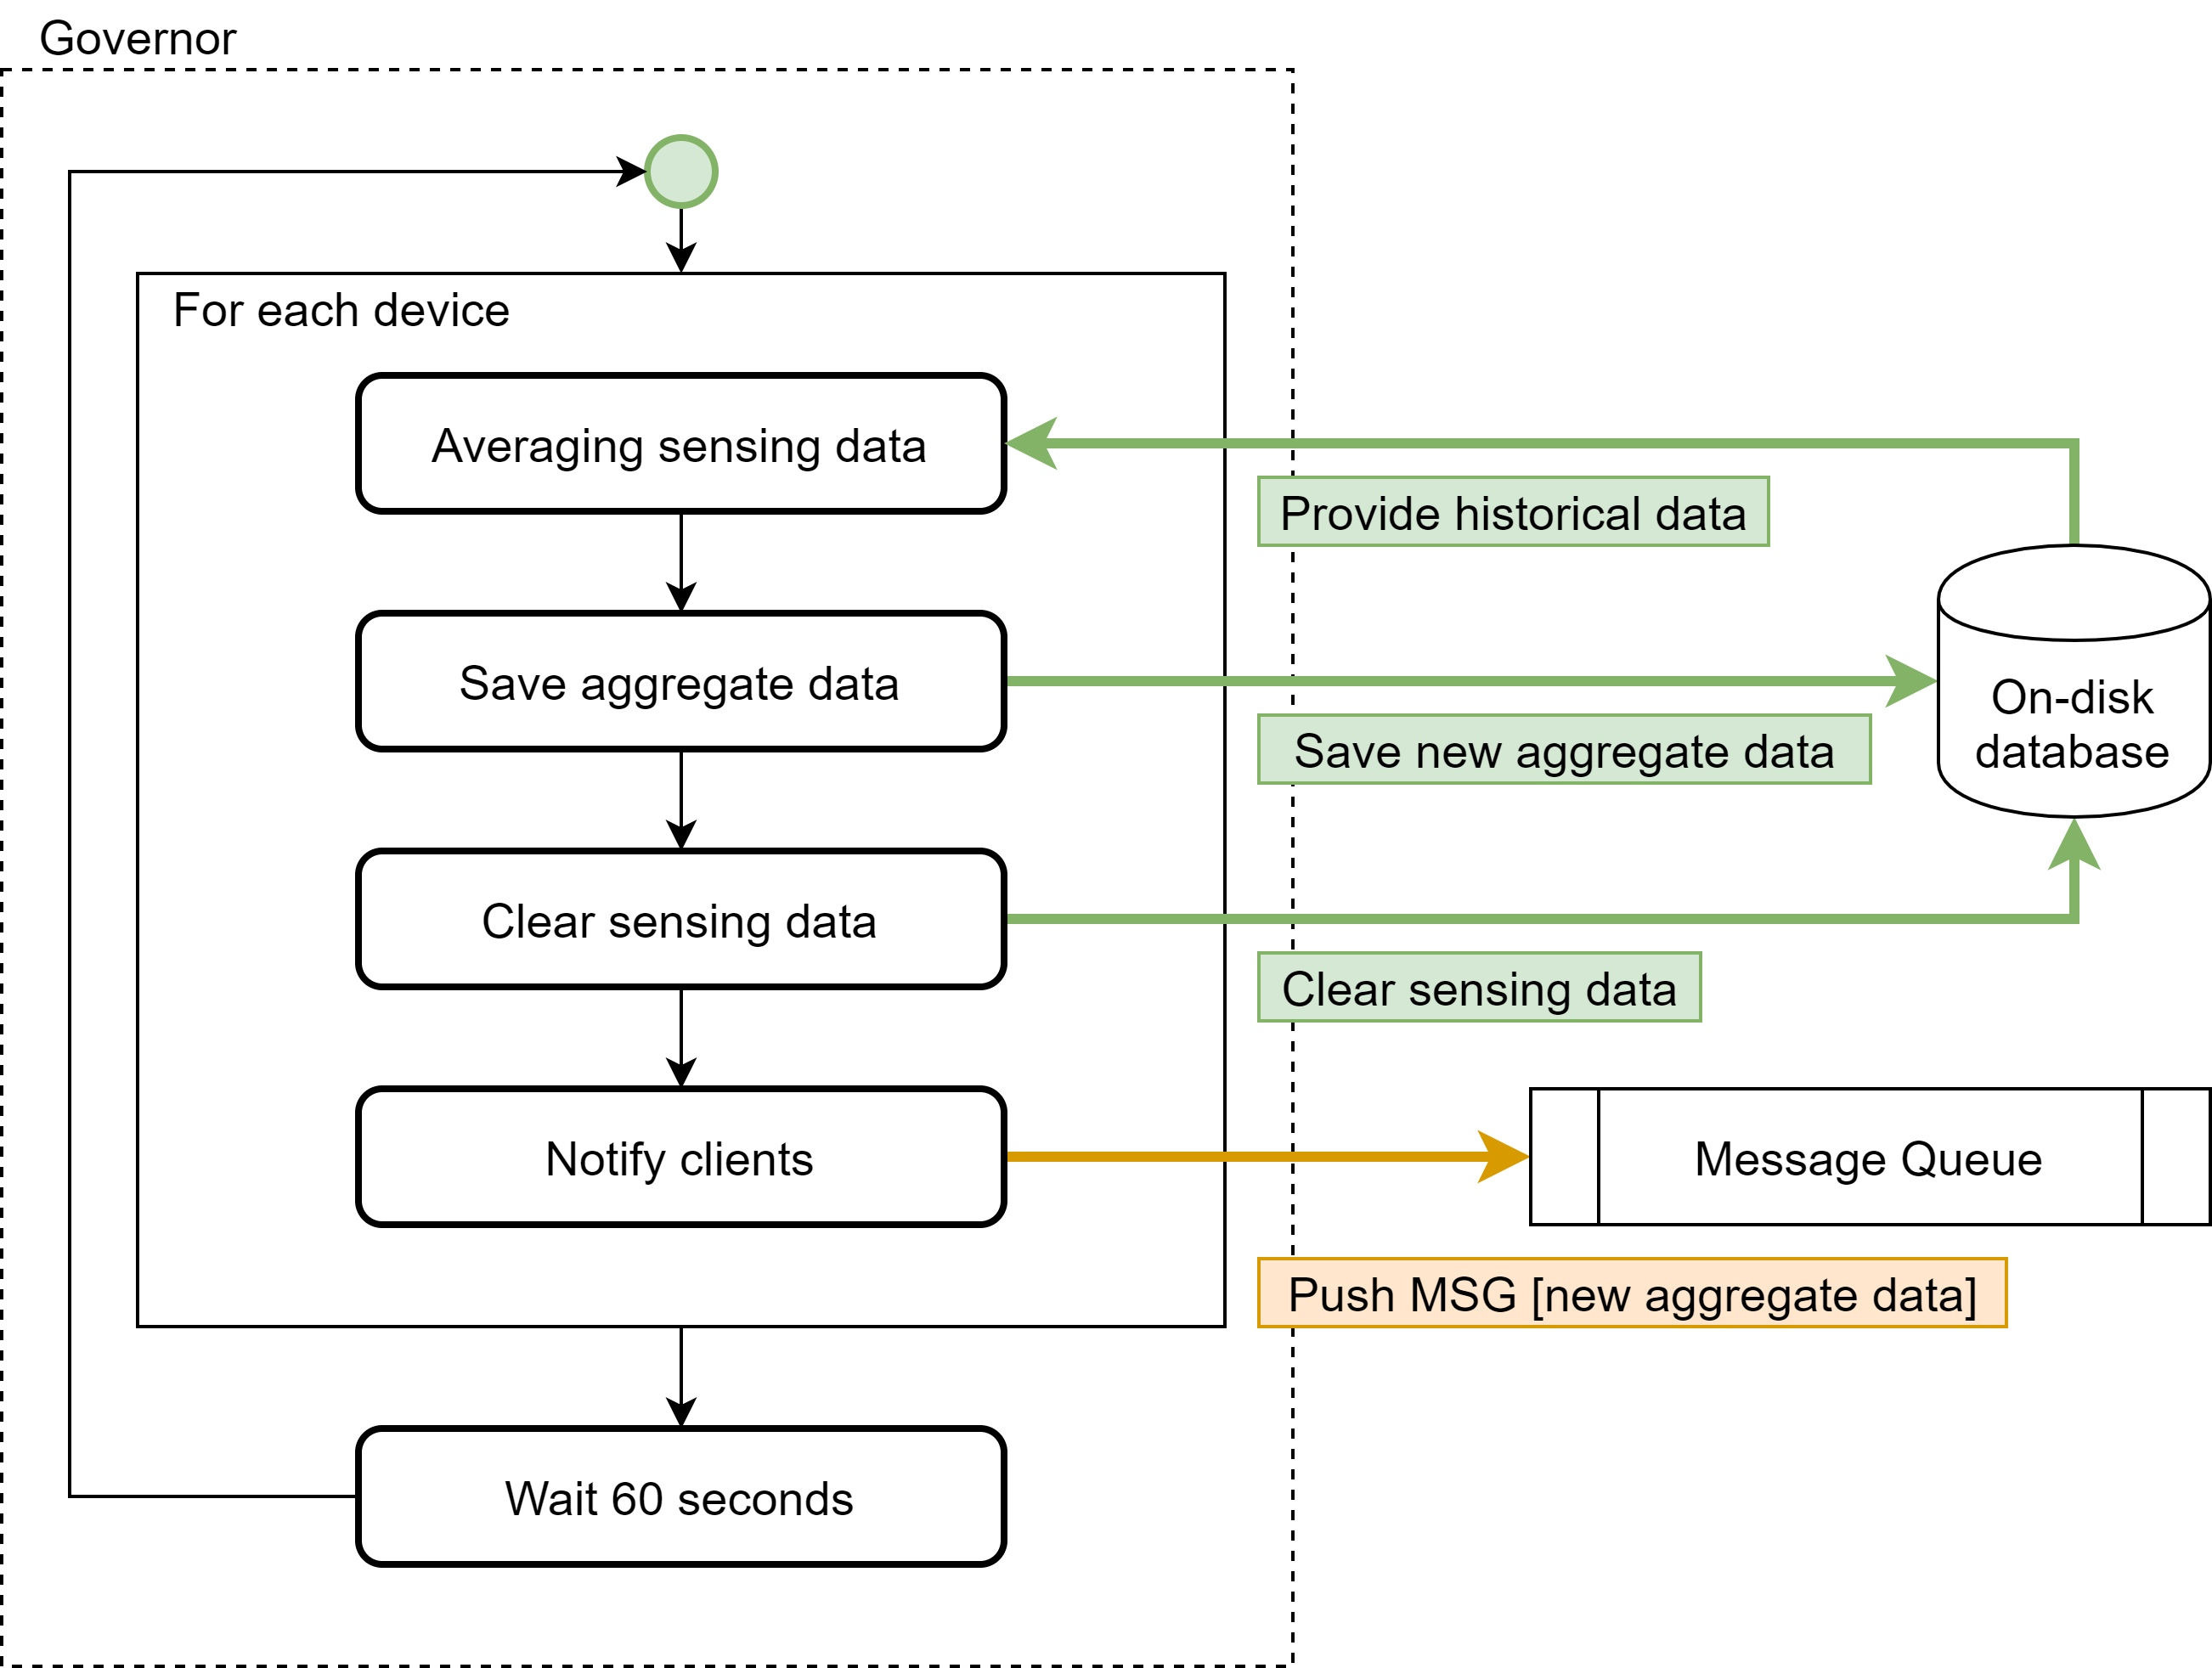
\includegraphics[width=\linewidth]{c4-governing.png}
	\caption{The governing process.}
	\label{fig:governing}
\end{figure}

\subsection{Context-aware load balancing}

Load balancing is an act of distributing load to different servers evenly to improve the overall performance. This is because it prevents the situation where a single server is overwhelmed by the load while other servers are experiencing starvation\footnote{Starvation in the context of computer system is a resource such as computation power that is being significantly underutilised.}. It is context-aware in the proposed system because the load balancer keeping track of the number of active connections a server has and direct the load to the server with the least amount of active connections. 

This is different to the conventional load balancers where it uses simple scheduling algorithms such as round-robin to dictate which server the load should be distributed to. The primary reason for using a custom scheduling logic is because the connections in the proposed system are persistent\footnote{The connection may last for a long time, and making many queries while it is connected.} while the connections in a typical system are one-off\footnote{The connection only query the system once and only once.}. That means, if a server is unfortunate enough that all of its active connections have very long lifespan, while connections in other servers have very short lifespan. The simple scheduling algorithm would continue to distribute the load to the server that still has many active connections due to the algorithm only cares about the order of the distribution not the actual load the server has. By being context-aware, the load balancer only distribute the load to the server with the least amount of active connections and the scenario above is avoided. 

Back to the proposed system, the context-aware load balancing process is shown in the figure \ref{fig:loadbalancing}. For a connecting client, it starts by querying the backend for a port it should connect to\footnote{A server usually sits behind a port in the computer system. Therefore, querying for a connection port is the same as querying for a particular server it should connect to.}. Then, the backend retrieves the connection count for each port from the in-memory database, find the one with the least amount of active connections, and return the port to the client. Once the client knows the port, it connects to the server at the port (the real-time composite component) and notify the server that it has connected. The server then realise it is a connect event and increment its internal connection count which keeps track of its own number of active connections. Finally, the server tells the backend that its active connection count has increased so that the backend is aware of the change and update the connection count associated with the port in the in-memory database. 

For a disconnecting client, which is caused by closing the web application or disconnected due to netowork issues. The disconnection would be detected by the server automatically and decrease the internal connection count. Like before, the server tells the backend that a connection has disconnected and the count is decreased. The backend reacts to it by also decreasing its connection count associated with the port that are stored in the in-memory database. 

Notice that both connecting and disconnecting would trigger a connection count update in the backend, and this allows the backend to keep track of the individual server load and distribute the load properly. 

The reason for using an in-memory database as oppose to storing the connection count in the server instance is because there are more than one backend instances in the proposed system. If all of them store the connection count in their own instance, then the connection count would not be updated correctly as the connection count synchronisation request is randomly distributed to any of the instances. As a result, each backend instance has a different connection count. Therefore, they need to share the connection count data using the in-memory database so all instances are accessing and updating the same connection count.  

\begin{figure}[!ht]
	\centering
	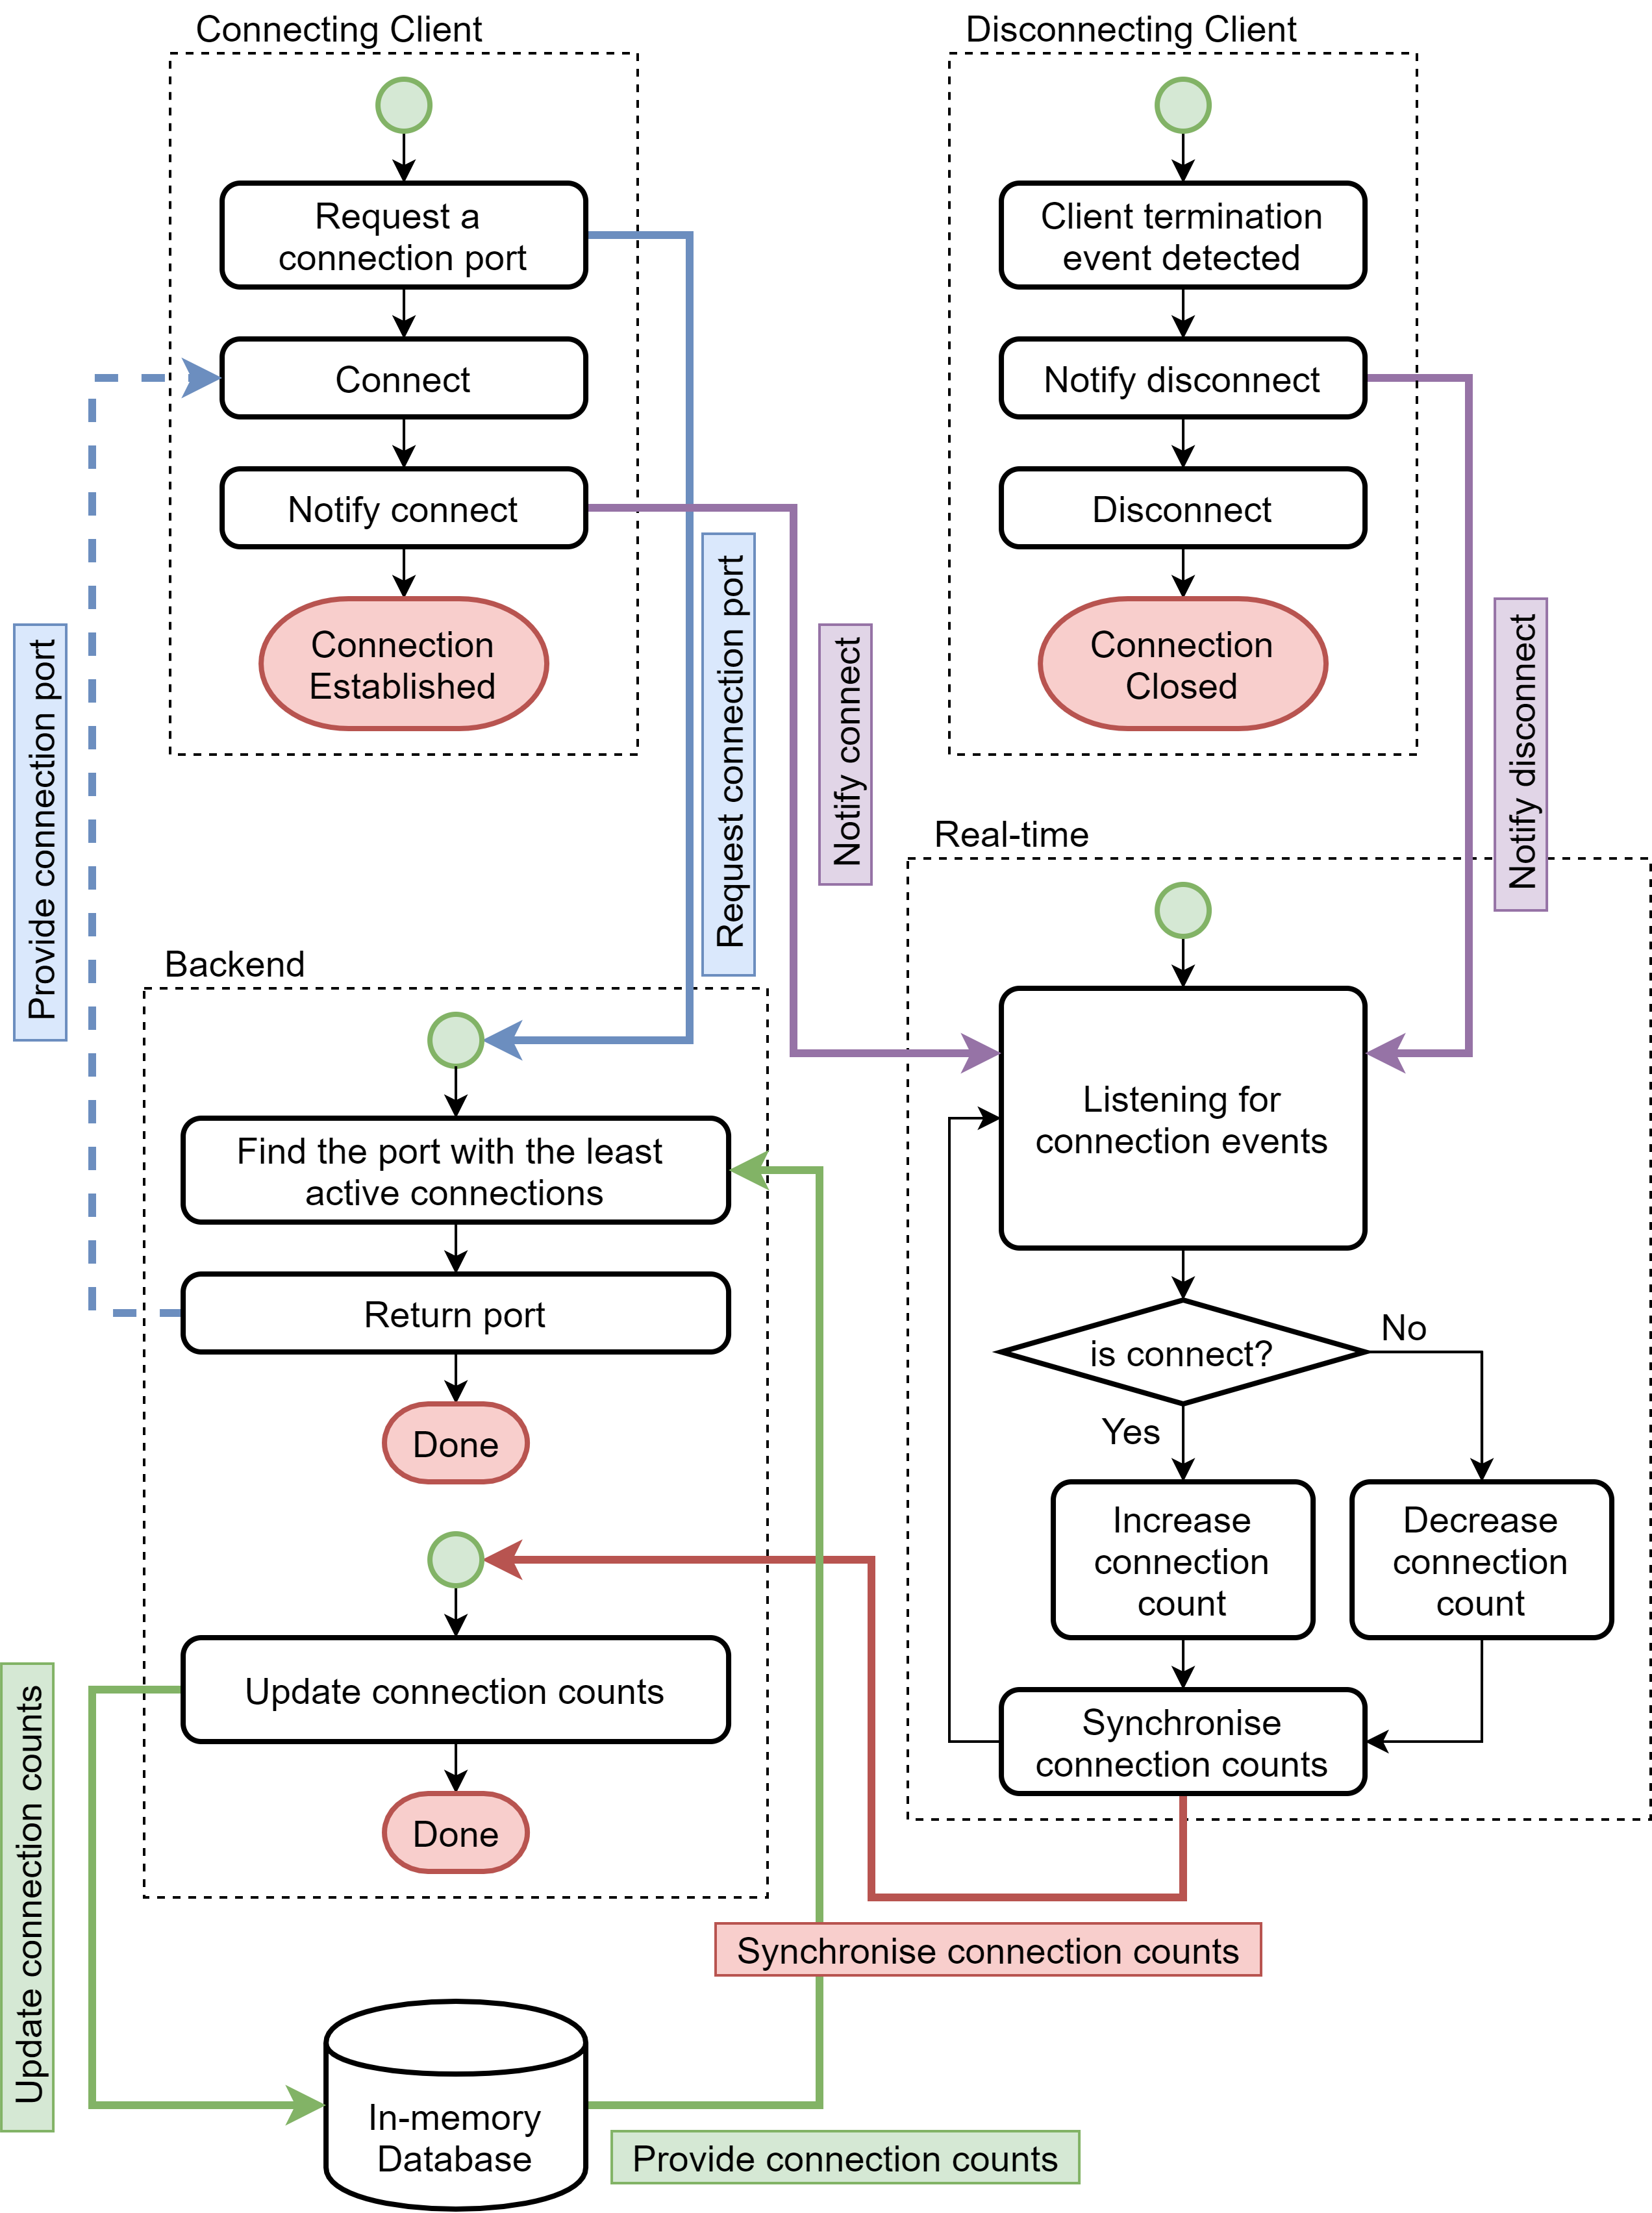
\includegraphics[width=0.95\linewidth]{c4-loadbalance.png}
	\caption{The context-aware load balancing process.}
	\label{fig:loadbalancing}
\end{figure}

\subsection{Data monitoring}

The data monitoring process is about showing the data on the client and the process is shown in the figure \ref{fig:monitoring}. Once the client is connected to a real-time server, the data monitoring process can begins. The first step is preloading the historical data from the backend which allows the user to view the previously recorded data for upto 4 hours immediatly after the client establishing the connection. During data preloading, the backend is fetching the data from the on-disk database and provide it to the client in the required format. Once the data preloading is done, the client starts listening for incoming data from the real-time server. Recall the new aggregate data is generated by the governor and the new sensing data is generated by the microcontroller, both of them produce a message into the message queue signifying a new piece of data is available. The consumer of both messages is the real-time server where it listens for the new data messages from the message queue and broadcast the new data to the relevant clients. The client takes the new data and add it to the visualisation. 

The benefit of using the real-time server is it significantly reduces the amount of backend access. Without the real-time server, the client have to periodically querying the backend regardless if there are new data or not. This is because there is no way to tell if a new piece of data is available at any given time. Assuming the querying rate is one query per second and there is only one client querying the backend. The periodic querying method would generate 60 queries per minute. By contrast, the real-time method only generates one and only one query, which is used for preloading the data. The load for the real-time method is shifted from backend to the real-time server and the number of messages from the real-time server is the number of times the microcontroller records the data. That means the worst case scenario is generating 60 data update messages per minute \footnote{The microcontroller records one sensing data every second.} to the client and the best case scenario is generating no data update as the microcontroller is not recording data. It is also worth noting that the cost of a query and data update is very different. A query involves accessing the on-disk database whereas the data update doesn't. Since accessing on-disk database is very slow by contrast, 60 real-time updates is more efficient than 60 queries.

\begin{figure}[!ht]
	\centering
	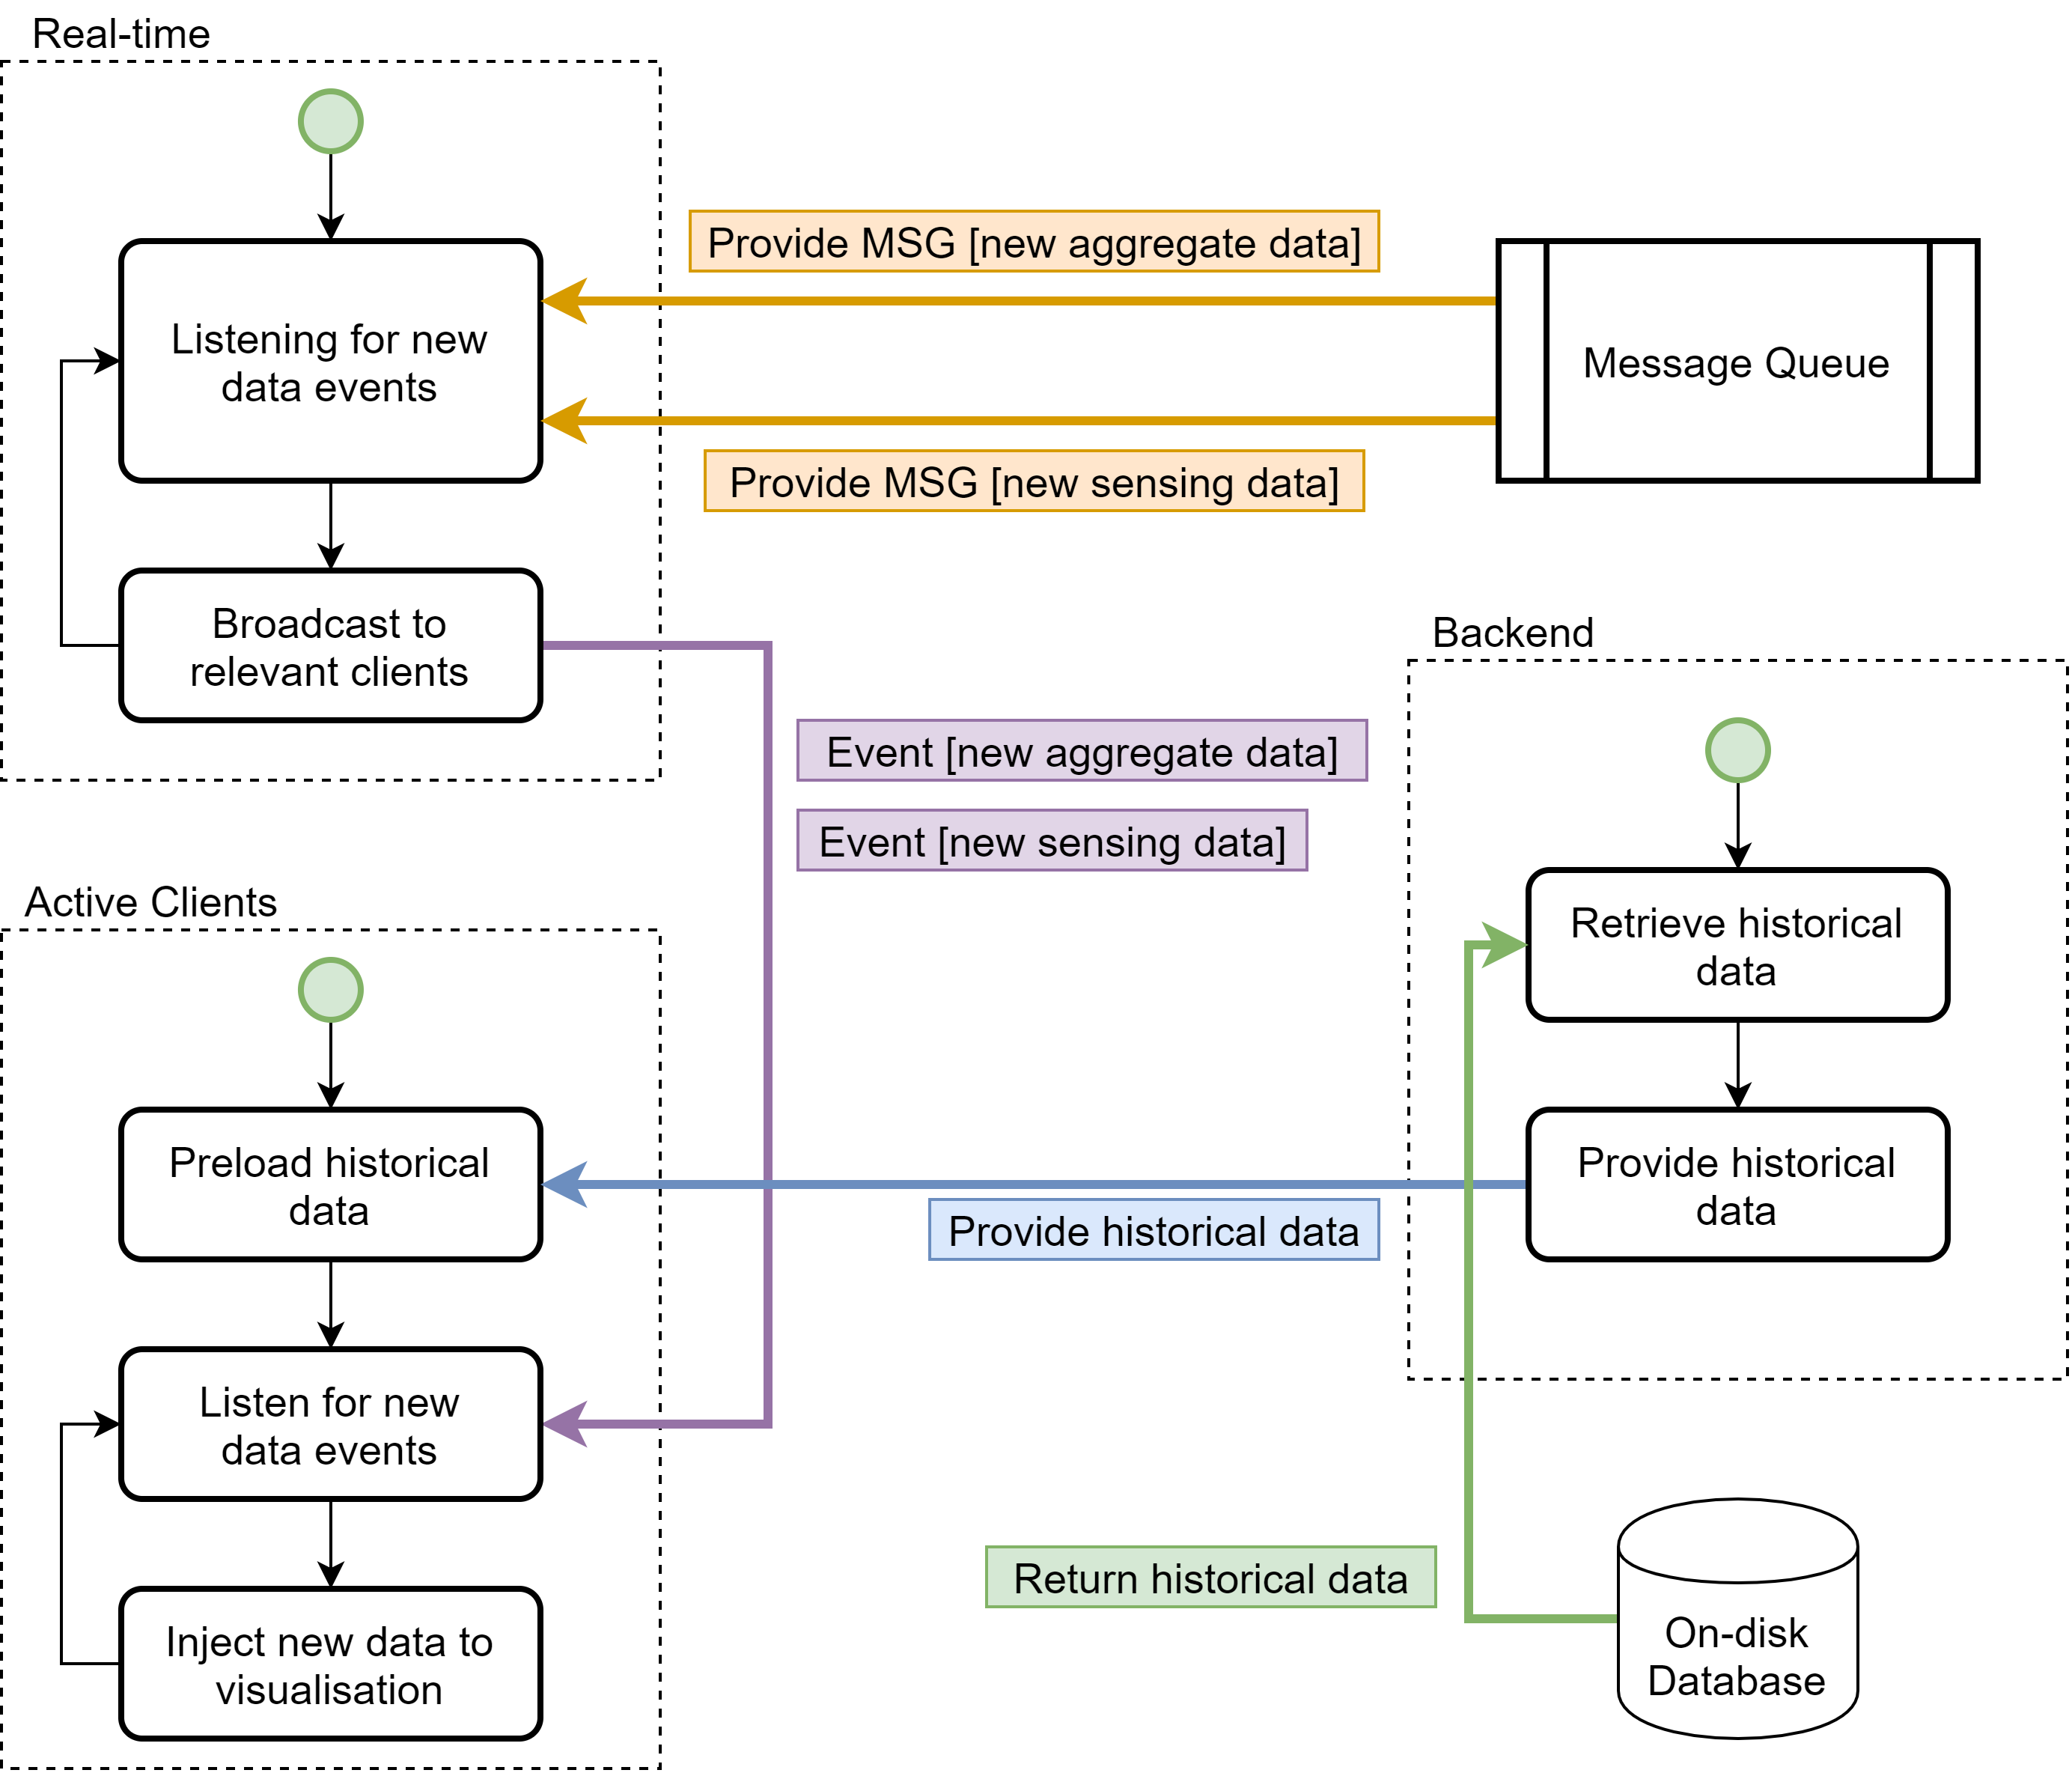
\includegraphics[width=\linewidth]{c4-monitoring.png}
	\caption{The data monitoring process.}
	\label{fig:monitoring}
\end{figure}

\subsection{Issuing command}

The process of issuing a command involves the user issuing a command through the user interface and queuing the command in the database for the microcontroller to retrieve and execute. The process is shown in the figure \ref{fig:issuing}. The process begins when the client sends the command to the backend, and then the backend enqueue the command inside the on-disk database. The order of the commands stored in the database must be maintained to ensure the correctness of the result after the microcontroller executes a series of commands.


\begin{figure}[!ht]
	\centering
	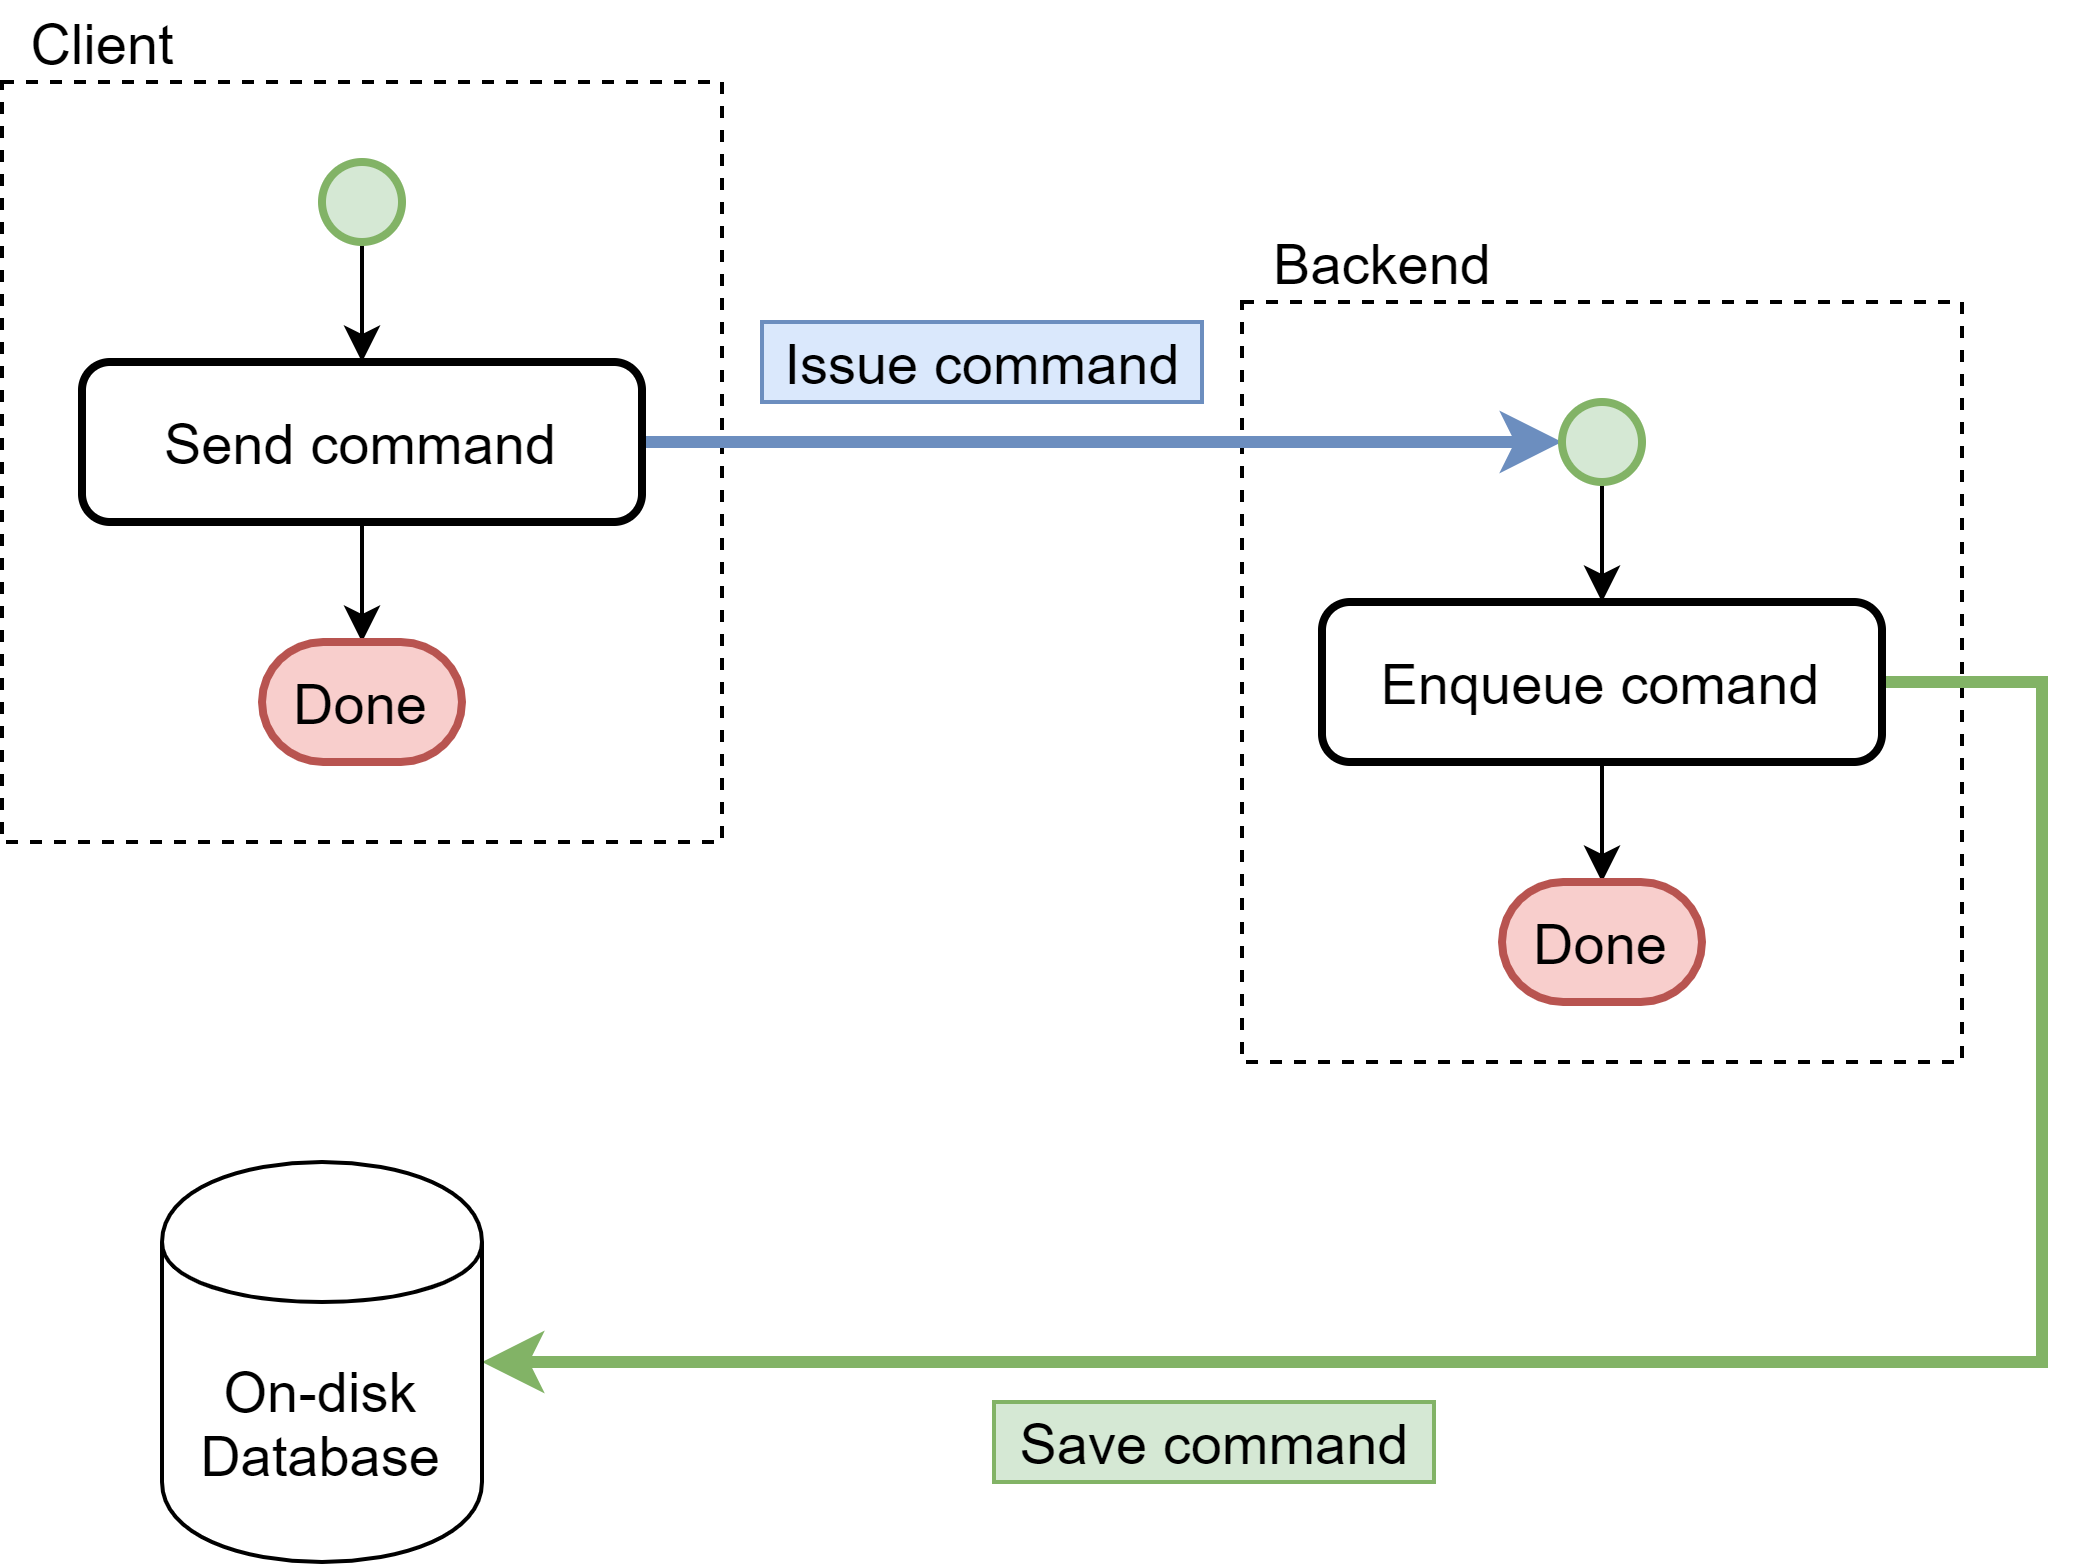
\includegraphics[width=\linewidth]{c4-issuing.png}
	\caption{The process of issuing a command.}
	\label{fig:issuing}
\end{figure}

\section{Low-level architecture}

In this section, the composite components shown in the top-level architecture are described in detail. 

\subsection{Remote sensing}
\label{sec:remoteSensing}
sdfsdf

\subsection{Backend}
\label{sec:backend}
sdfsdf
\subsection{Frontend}
\label{sec:frontend}
sdfsdf
\subsection{Real-time}
\label{sec:realtime}
sdfsdf

\subsection{Simulator}
\label{sec:simulator}
sdfsdf
\subsection{Client}
\label{sec:webClient}


\end{document}